\section{Clover-based prototype}

While our insight and approach is general, in order to demonstrate its
practicality we prototype it in the context of Clover~\cite{clover}, a
disaggregated key/value store.  Hence, we begin with a brief overview
of the relevant aspects of Clover's design for the uninitiated.

Clover maximizes read performance by separating key/value metadata
from the datapath, which is implemented as a linked list of value
updates that the authors term a \emph{chain}. Clients issue lock-less
value reads at the end of the chain directly to passive remote memory
servers and issue opportunistic writes guarded by an RDMA
compare-and-swap (c\&s) operation to ensure consistency.  When writes
(i.e., c\&s operations) succeed clients update metadata severs lazily
with the new location of the end of the chain (as any concurrent
writes to the same location will fail the comparison). If reads or
writes fail because clients did not access the current end of the
chain they concurrently request fresh metadata and traverse the
chain in remote memory to find the new end (a processes
known as \emph{chain walking}). The authors show this approach obtains
extremely high throughput with read-heavy workloads as updates are
rare and clients enjoy unfettered access to remote memory. In contrast
they find that placing a metadata coordinator in the datapath becomes
a bottleneck at only a fraction of their achievable throughput.

\begin{figure}
    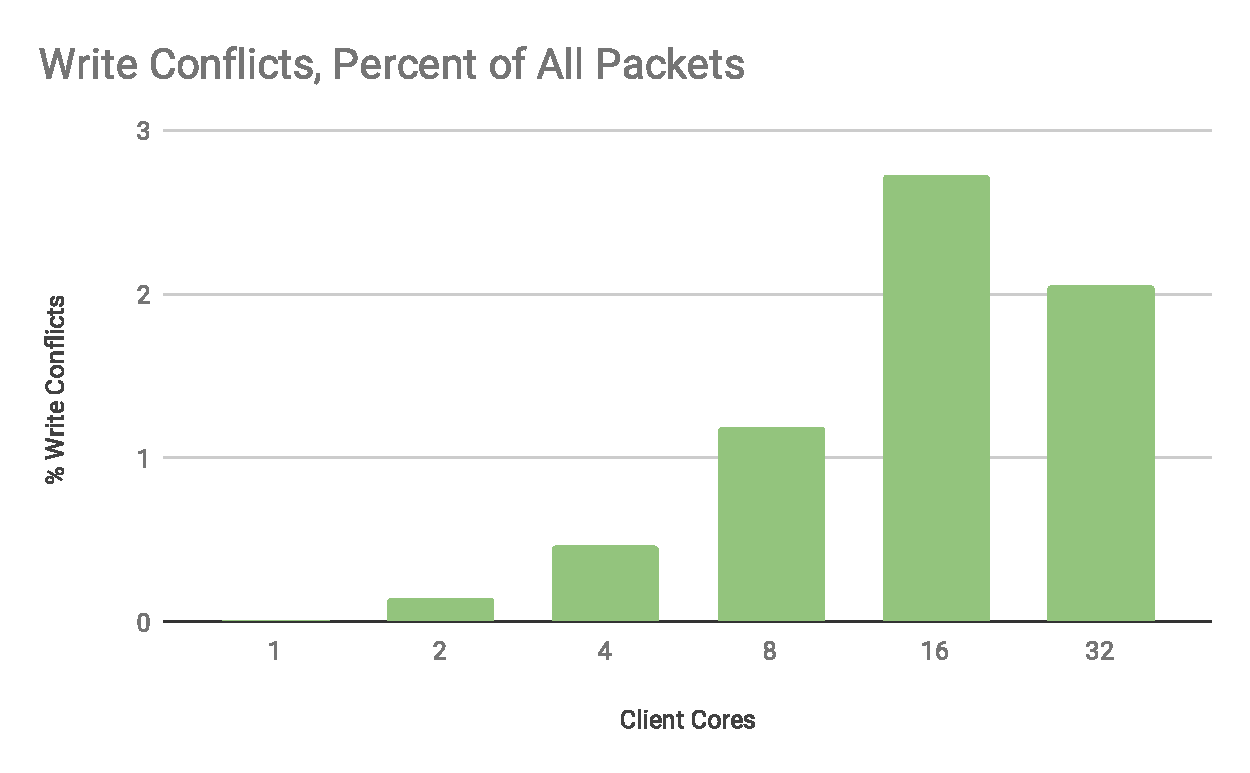
\includegraphics[width=0.45\textwidth]{fig/write_conflicts.pdf}
    \caption{Clover write conflicts grow with the number of clients
    (50\% write Zipf 0.99 distribution)\todo{redo with 64 cores and
    writes only}}
    \label{fig:conflicts}
    \vskip -0.5em
\end{figure}

In the presence of writes, however, Clover's throughput decreases due
to contention. When concurrent writes update the same key a race
occurs to write at the end of the chain. Write operations require two
messages, a data update (i.e., RDMA WRITE) and guard (RDMA c\&s) which
updates the chain to point to the new value. During this two-RTT
operation any concurrent write to the same key will cause a conflict.
The slower writers will fail the guard, and must retry their write after
walking the chain through remote memory or by getting an update from the
metadata server.  On write-heavy workloads these race conditions
happen frequently as illustrated in Figure~\ref{fig:conflicts}, which
leads to a sharp decrease in throughput.

We propose a middle ground between Clover and a centralized approach.
Our insight is that by using data-structure-specific knowledge and
caching write locations in the network, conflicting writes can be
resolved at line rate on the data path.  Using Clover as a platform to
prove our concept we design a middle-box algorithm which intercepts
Clover's RDMA read and write/c\&s requests, caches a small amount (64 bytes
per key) of structural metadata, and resolves write conflicts by
adjusting the destination RDMA virtual address of the writes and c\&s
guards. Our algorithm is implemented using DPDK, but is designed to
have low memory and computational overhead making it ideal for network
devices such as programmable switches.


%% The high level pitch about remote memory.
%Far memory projects typically have a remote CPU which is used to
%coordinate access to remote resources (cite all object systems). In a
%disaggregated system there is no remote CPU, therefore the coordination
%of reads and writes to remote locations must be done locally. For
%performance local caches of remote resources can be used to organize
%access to remote resources. For data structures which require
%consistency this creates a problem as stale caches can lead to data
%structure corruption.

